\documentclass[12pt]{article}
\usepackage{tikz}
\usepackage{float}
\begin{document}
\title{Computer Science 118, Homework 3}
\date{November 15th, 2018}
\author{Michael Wu\\UID: 404751542}
\maketitle

\section*{Problem 1}

\paragraph{a)}

There is no need for a padding character to create a packet that is at least a minimum size. Thus we can assume that each packet only contains valid data,
and no length field is necessary in the Ethernet header either.

\paragraph{b)}

No, since small packets are valid in Nethernet and this is not an error.

\paragraph{c)}

Yes, since large packets still exist, Nethernet would behave the same as Ethernet in detecting collisions for packets of size greater than the minimum packet size.
For example, assume \(A\) sends a 64 byte packet. At the same time \(B\) sends a 64 byte packet. Without regular detection methods, \(A\) will not see any transmission
during the wait time as it is still sending its own packet. Thus no collision is detected when there is one. So we need the regular method of collision detection as well.

\paragraph{d)}

Assume that \(A\) sends a 1 byte packet and \(B\) sends a 64 byte packet. \(B\) would not detect a collision because the time to send 1 byte is smaller than the jamming time.
So \(A\) would detect a collision since it receives a transmission within the wait period, while \(B\) does not detect a collision.

\paragraph{e)}

Let there be three nodes on the Nethernet. Two send short frames, detect collision, and retransmit. However, the third would detect no overlap between the transmissions. In this
case the protocol would not indicate a collision if the third node does not transmit anything. So the third node would receive duplicate frames.

\section*{Problem 2}

\paragraph{a)}

\begin{figure}[H]
    \begin{center}
        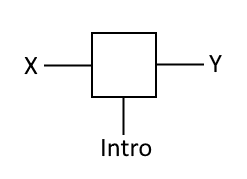
\includegraphics[width=2.5in]{problem2.png}
    \end{center}
\end{figure}

Consider the setup above. Each one of \(X\), \(Y\), and \(INTRO\) reside on a separate Ethernets and are connected through the bridge. First \(X\) sends a frame to \(INTRO\). The bridge learns
that \(X\) is on the left network. \(INTRO\) forwards the frame and replaces the destination with \(Y\). But once the bridge receives the updated frame, it will think that \(X\) is on the bottom
network since the source is not changed by \(INTRO\). When \(Y\) attempts to send to \(X\), the bridge will send the frame to the bottom LAN, which will drop the frame since \(X\) does not reside there.
So the protocol fails since the frame is not delivered correctly.

\paragraph{b)}

\(INTRO\) should send a frame back to \(X\) saying that \(Y\) corresponds to \(H\). Then the response frame should have \(INTRO\) as the source and \(X\) as the destination. Afterwards \(X\) can update its
original frame and send directly to \(Y\). This ensures that each frame is sent with the correct source, so bridging would not interfere with the protocol.

\section*{Problem 3}

First \(B\) will send an ARP request, which each node on the Ethernet receives. This request is discarded by everyone except \(A\), who replies and lets \(B\) know that it has the data link address of all 1's.
Then \(B\) will send a packet using this multicast address. Again everyone receives this packet, but everyone except \(A\) forwards the packet since the IP addresses would not match. Each time the packet is forwarded,
it gets sent to the multicast address and pings back and forth infinitely among \(B\), \(C\), \(D\), and \(E\).

If the bridge were replaced with an IP router, the router would know that the upper end nodes do not have the same IP prefix as \(A\), so they would not receive the packet. Thus only \(B\) and \(C\) would repeatedly
forward the packet between each other, which is better than in the first scenario but still bad. \(C\) and \(D\)'s LAN would not be congested, but the bottom one would be.

\section*{Problem 4}

Add a third field that is the minimum max packet size. When a router \(R\) tells another router \(S\) the distance to the destination \(D\), take the minimum of the current minimum max packet size between
\(R\) and \(D\) and the max packet size between \(R\) and \(S\) and send it along with the distance information. The router \(S\) still picks a distance based on the minimum distance calculation, but each
minimum distance calculation also has a given max packet size associated with it. Thus \(S\) will automatically know the minimum max packet size on the shortest path to \(D\).

\end{document}